\documentclass{article}
\usepackage{tikz}
\usetikzlibrary{shapes.geometric}

\begin{document}

\begin{figure}[h]
    \centering
    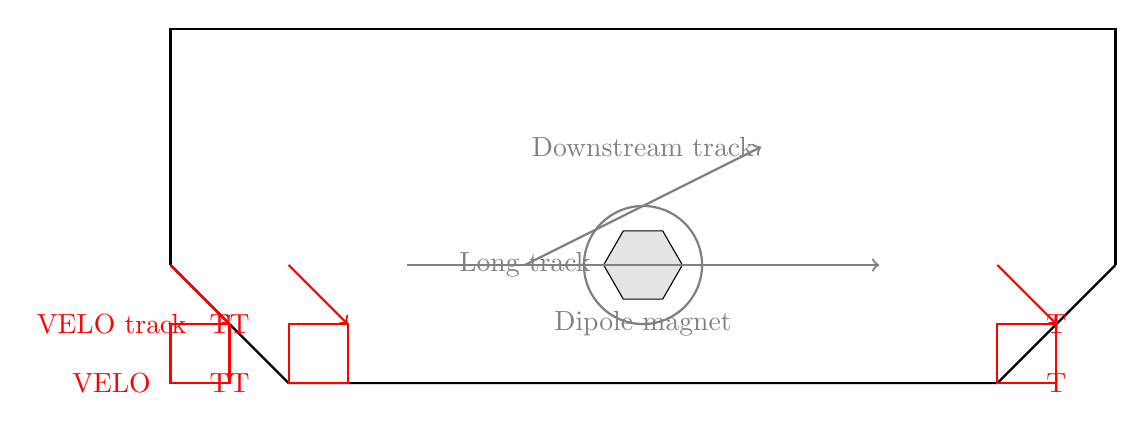
\begin{tikzpicture}[scale=1.5]

        % Draw the main structure
        \draw[thick] (-4,-2) -- (-4,0) -- (4,0) -- (4,-2);
        \draw[thick] (-4,-2) -- (-3,-3) -- (3,-3) -- (4,-2);

        % Draw the VELO track
        \draw[->, thick, red] (-4,-2) -- (-3.5,-2.5);
        \node at (-4.5,-2.5) [red] {VELO track};

        % Draw the TT track
        \draw[->, thick, red] (-3,-2) -- (-2.5,-2.5);
        \node at (-3.5,-2.5) [red] {TT};

        % Draw the Dipole magnet
        \node[regular polygon, regular polygon sides=6, minimum size=1cm, draw, fill=gray!20] at (0,-2) {};

        % Draw the T track
        \draw[->, thick, red] (3,-2) -- (3.5,-2.5);
        \node at (3.5,-2.5) [red] {T};

        % Draw the Long track
        \draw[->, thick, gray] (-2,-2) -- (2,-2);
        \node at (-1,-2) [gray] {Long track};

        % Draw the Downstream track
        \draw[->, thick, gray] (-1,-2) -- (1,-1);
        \node at (0,-1) [gray] {Downstream track};

        % Draw the VELO detector
        \draw[thick, red] (-4,-2.5) -- (-3.5,-2.5) -- (-3.5,-3) -- (-4,-3) -- cycle;
        \node at (-4.5,-3) [red] {VELO};

        % Draw the TT detector
        \draw[thick, red] (-3,-2.5) -- (-2.5,-2.5) -- (-2.5,-3) -- (-3,-3) -- cycle;
        \node at (-3.5,-3) [red] {TT};

        % Draw the T detector
        \draw[thick, red] (3,-2.5) -- (3.5,-2.5) -- (3.5,-3) -- (3,-3) -- cycle;
        \node at (3.5,-3) [red] {T};

        % Draw the Dipole magnet
        \draw[thick, gray] (0,-2) circle (0.5);
        \node at (0,-2.5) [gray] {Dipole magnet};

    \end{tikzpicture}
    \caption{Schematic view of the different track types relevant for this paper, along with the used tracking detectors for these track types, showing the VELO detector, the TT detector, the magnet and the downstream tracking stations (T). The names of the tracking detectors along with the positioning of the magnet are indicated below the figure.}
    \label{fig:track_types}
\end{figure}

\end{document}